\section{Manage your local environment}
\subsection{How conda works}
\begin{frame}[<+->]{Example of R and package installation}{Conda use}
\begin{itemize}
	\item Separate each application in it own environment 
\includegraphics[width=0.1\textwidth]{conda_logo.pdf}
	\item A tool version = a conda environment
	\item Create a new environment for a new tool version, an analysis...
\end{itemize}
\onslide<1->{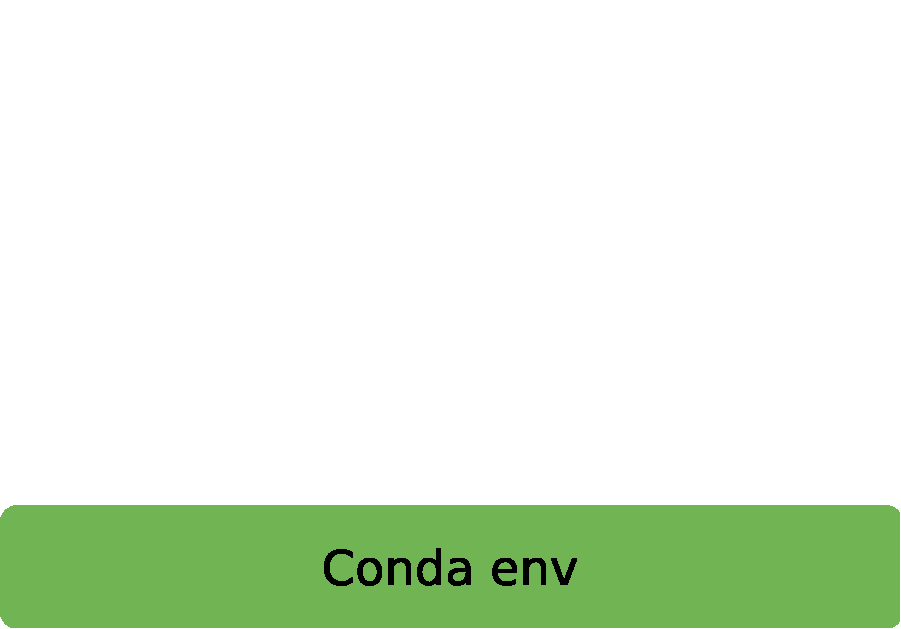
\includegraphics[width=0.3\textwidth]{conda_env_5.pdf}}
\onslide<2->{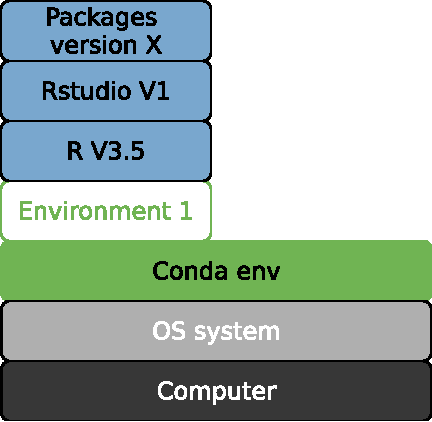
\includegraphics[width=0.3\textwidth]{conda_env_6.pdf}}
\onslide<3->{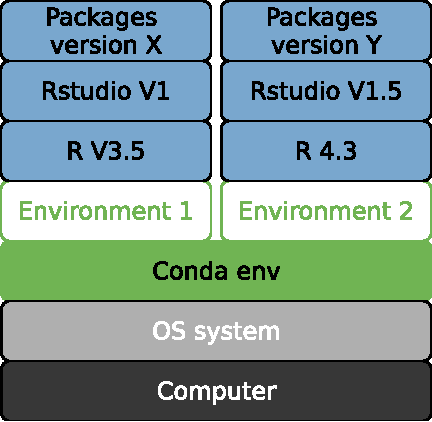
\includegraphics[width=0.3\textwidth]{conda_env_7.pdf}}
\end{frame}
